\section{Non-Text Format Templates}
This section meant to provide template figures, tables, equations, and references that can be copied and pasted to other parts of the document in a simple manner.

Figures will behave as Fig. \ref{fig: test}. Note that the placement may seem random, but is chosen by \LaTeX\ automatically.
\begin{figure}[!ht]
\centering
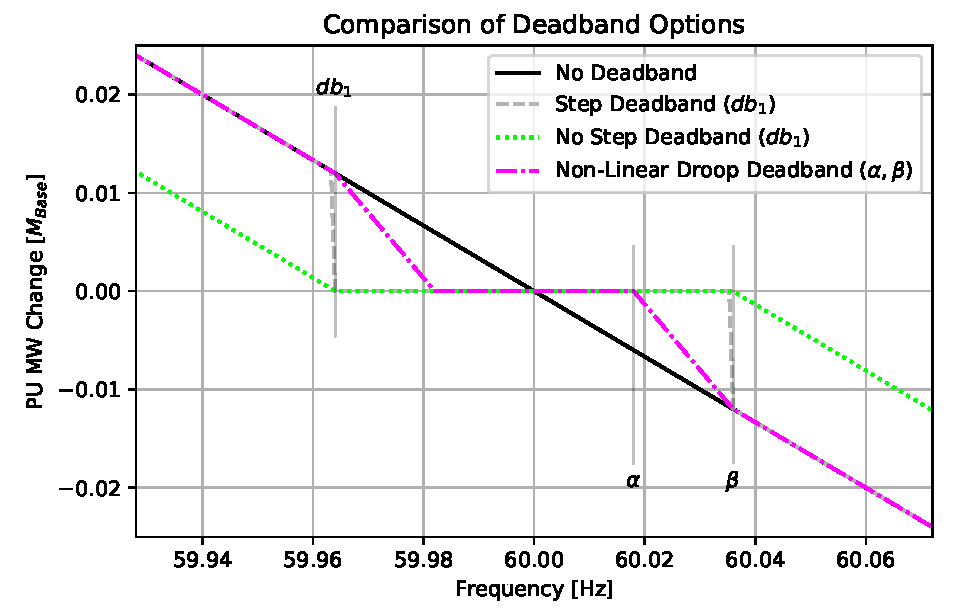
\includegraphics[width=\linewidth]{figures/dbAction3}
\caption{Testing of figure format.}
\label{fig: test}
\end{figure}


The default IEEE table example leaves something to be desired that is fulfilled by using the \verb|booktabs| package.
This is shown in Table \ref{tab: test2}.
% Testing of external table build for \input later
% Uses the IEEE table format guidelines
\begin{table}[!ht]
	\caption{Generic governor model parameters.}
	\label{tab: test2}
	\centering
	\begin{tabular}{@{} C{2cm} S[table-format=2.2] S[table-format=2.2] S[table-format=2.2] @{}} 	
		\toprule % @ signs to remove extra L R space
		\text{Parameter}	&	\text{Steam}	&	\text{Hydro}	&	\text{Gas}	\\		
		\midrule		
			Ts	&	0.04	&	0.40	&0.50\\
			Tc	&	0.20	&	45.00	&10.00\\
			T3	&	0.00	&	5.00	&4.00\\
			T4	&	1.50	&	-1.00	&0.00\\
			T5	&	5.00	&	0.50	&1.00\\
		\bottomrule
	\end{tabular}

\end{table}

Equations are entered as one may normally do in a \LaTeX\ situation and referenced as (\ref{eq: TestEq1}) and (\ref{eq: TestEq2}).
\begin{align}
f_{ss} &= f_{ref}+\Delta f = f_{ref} + \dfrac{\Delta P}{S_{Base}\beta}  \label{eq: TestEq1}\\
\beta &= \sum_{i=1}^{N} \dfrac{1}{R_i \frac{S_{Base}}{M_{Base, i}} } \label{eq: TestEq2}
\end{align}

References are only included if cited. For instance \cite{Kundur} or \cite{DonnellyVoltageControl} are randomly cited. Note that the sorting order is set to \verb|none|, which lists references in order cited.
